\documentclass[12pt]{article}
\usepackage{graphicx} % Required for inserting images
\usepackage{caption}
\usepackage[top=0.1in, bottom=0.7in, left=1in, right=1in]{geometry} % Sets all margins to 1 inch
\usepackage{titlesec} % Adjust section title fonts

\title{Is Florida getting warmer?}
\author{Laiyin Zhou}
\date{November 2024}

\titleformat{\section}
    {\normalfont\large\bfseries}{\thesection}{1em}{} % set the section title font size to large

\begin{document}
    \maketitle

    \section{Introduction}
    This study examines the relationship between years and annual mean temperatures in Key West, Florida. It is hypothesized that Florida’s annual mean temperature has been increasing over the years.

    \section{Methods}
    The relationship between year and annual mean temperature was analyzed using Pearson’s correlation coefficient. Since annual temperatures are sequentially dependent, a permutation test was performed to assess the statistical significance of the observed correlation. In the test, the annual temperature sequence was randomly reshuffled 10,000 times and the correlation coefficient was recalculated for each permutation. An approximate p-value was calculated as the proportion of permuted correlation coefficients greater than or equal to the observed correlation coefficient.
    
    \section{Results}
    The observed correlation coefficient between year and annual mean temperature is 0.53, with an approximate p-value of 0, indicating a statistically significant positive relationship. This suggests that the observed increase in temperatures is unlikely due to random variation and provides evidence that Florida is getting warmer (Figure~\ref{fig:pdfimage}).
        
    % Insert the PDF image
    \begin{figure}[h!]
        \centering
        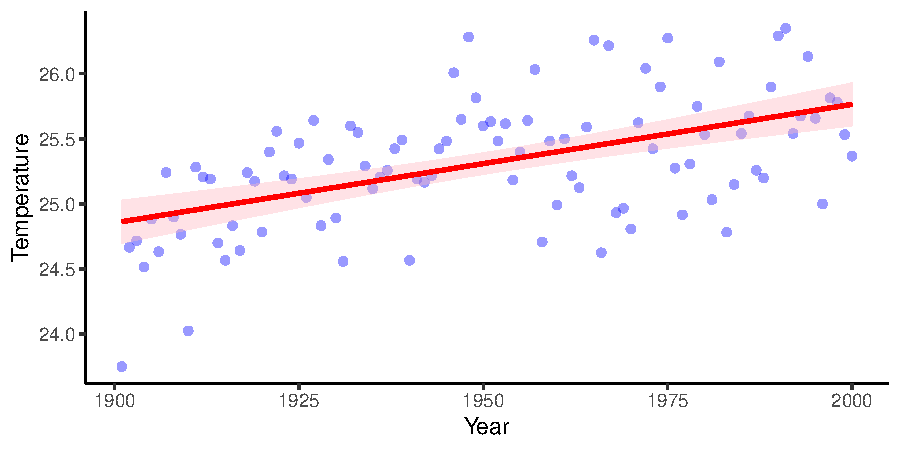
\includegraphics[width=0.8\textwidth]{../results/Florida.pdf}  % Adjust width as needed
        \caption{Relationship between year and temperature in Key West, with 95\% confidence interval. Each point represents an annual mean temperature.}
        \label{fig:pdfimage}
    \end{figure}

\end{document}
